
\section{Evaluation}
\label{sec:evaluation}
In this section, we present an experimental evaluation of \projecttitle based on the implementation described in  $\S$\ref{sec:implementation}. 
Our evaluation answers the following questions.


\begin{figure}[t]
\centering
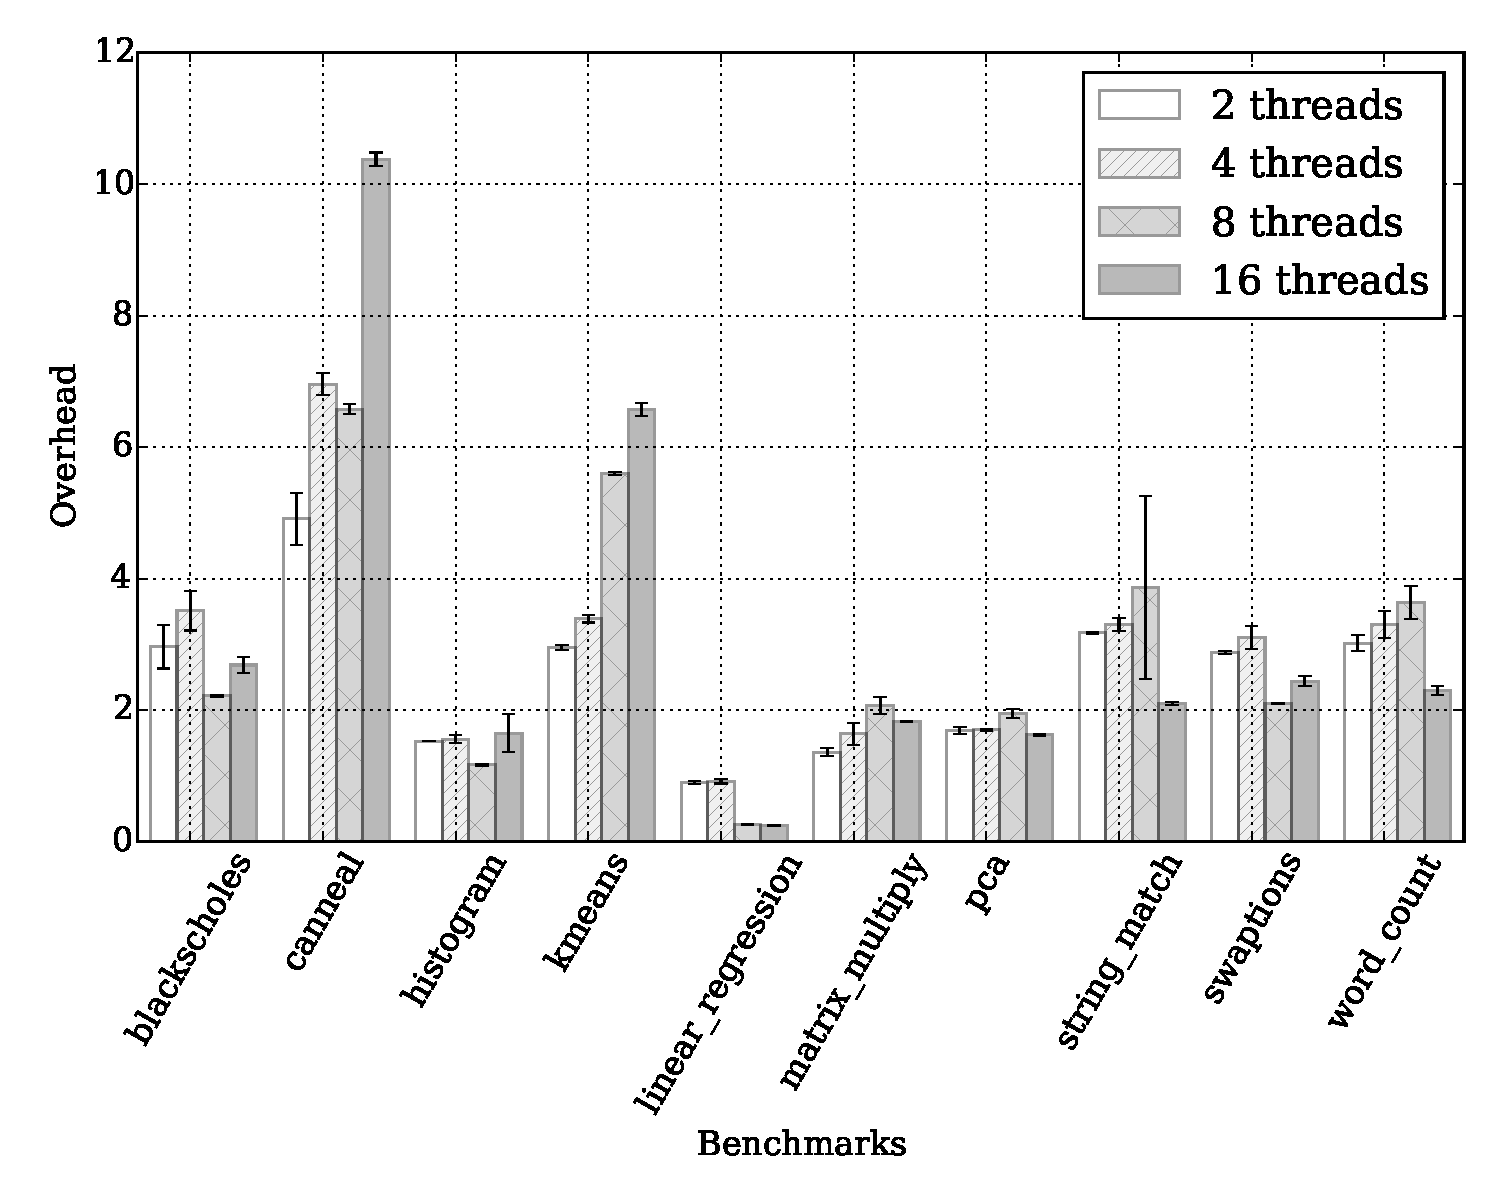
\includegraphics[scale=0.46]{figure/benchmarks/times-inspector.pdf}
\caption{Performance overhead  over native execution with increasing number of threads.}
\label{fig:overheads}
\end{figure}


\begin{itemize}
\item What performance overheads does \projecttitle impose for recording the provenance graph? ($\S$\ref{subsec:overheads})
\item What are the sources for these overheads? ($\S$\ref{subsec:performance-overheads-breakdown})
\item How do these overheads scale with increase in the size of input data? ($\S$\ref{subsec:data-sizes-overheads})
\item What are the space overheads for the CPG? ($\S$\ref{subsec:overheads-breakdown})
\end{itemize}

%Before answering these questions, we first describe the experimental setup used for the evaluation.


\subsection{Experimental Setup}


\myparagraph{Experimental platform} We used an Intel Xeon processor based on Broadwell micro-architecture
as our host machine. The
host system consists of $8$ cores ($16$ hyper-threads) of Intel(R) Xeon(R) CPU Processor D-$1540$
($12$M Cache, $2.00$ GHz) and $32$ GB of DRAM main memory. The host
machine is running Linux with kernel $4.3.0$ in $64$-bit mode. 
%When varying the number of threads, we also regulate the numbers of active cpu cores.
%No additional core was provided for Perf.


%\myparagraph{Applications and dataset}  We evaluated \projecttitle using two multithreaded benchmark suites: Phoenix $2.0$~\cite{phoenix} and PARSEC $3.0$~\cite{parsec}. 

\myparagraph{Applications and dataset}  We evaluated \projecttitle using applications from two multithreaded benchmark suites: Phoenix 2.0 \cite{phoenix} and PARSEC 3.0 \cite{parsec}. Table~\ref{tab:apps} lists the applications used for the evaluation along with the input data and benchmark parameters.
%


\myparagraph{Performance metrics: Time and Work}  For each run, we consider two types of measures: \emph{time} and
 {\em work}.  Time refers to the amount of (end-to-end)
run-time to complete the parallel computation.  Work refers to the total amount of
computation performed by all threads and is measured as the overall CPUs utilization for all threads. 
%as the total run-time of all threads. 
Both metrics are important
and complementary: time measurements reflect the end user perceived latency,
whereas work measurements assess the overall resource (CPU) utilization.


\myparagraph{Measurements} All applications were compiled using
GCC $5.2.1$ compiler with {\tt -o3} optimization flag. For all
measurements, we report the average over $6$ runs with minimum and maximum values
discarded (truncated mean).

 We measured work and time numbers for both \pthreads and \projecttitle executions. For time measurements, we report the run-time comparison between the native {\tt pthreads} execution, and \projecttitle execution.   To measure work, we used the CPU accounting controller in {\tt cgroups} to account the CPU usage of all threads. 

Finally, the log produced by
{\tt perf} was written to {\tt /tmp} on {\tt tmpfs} to allow high throughput.
%For all experiments,  

\begin{figure}[t]
\centering
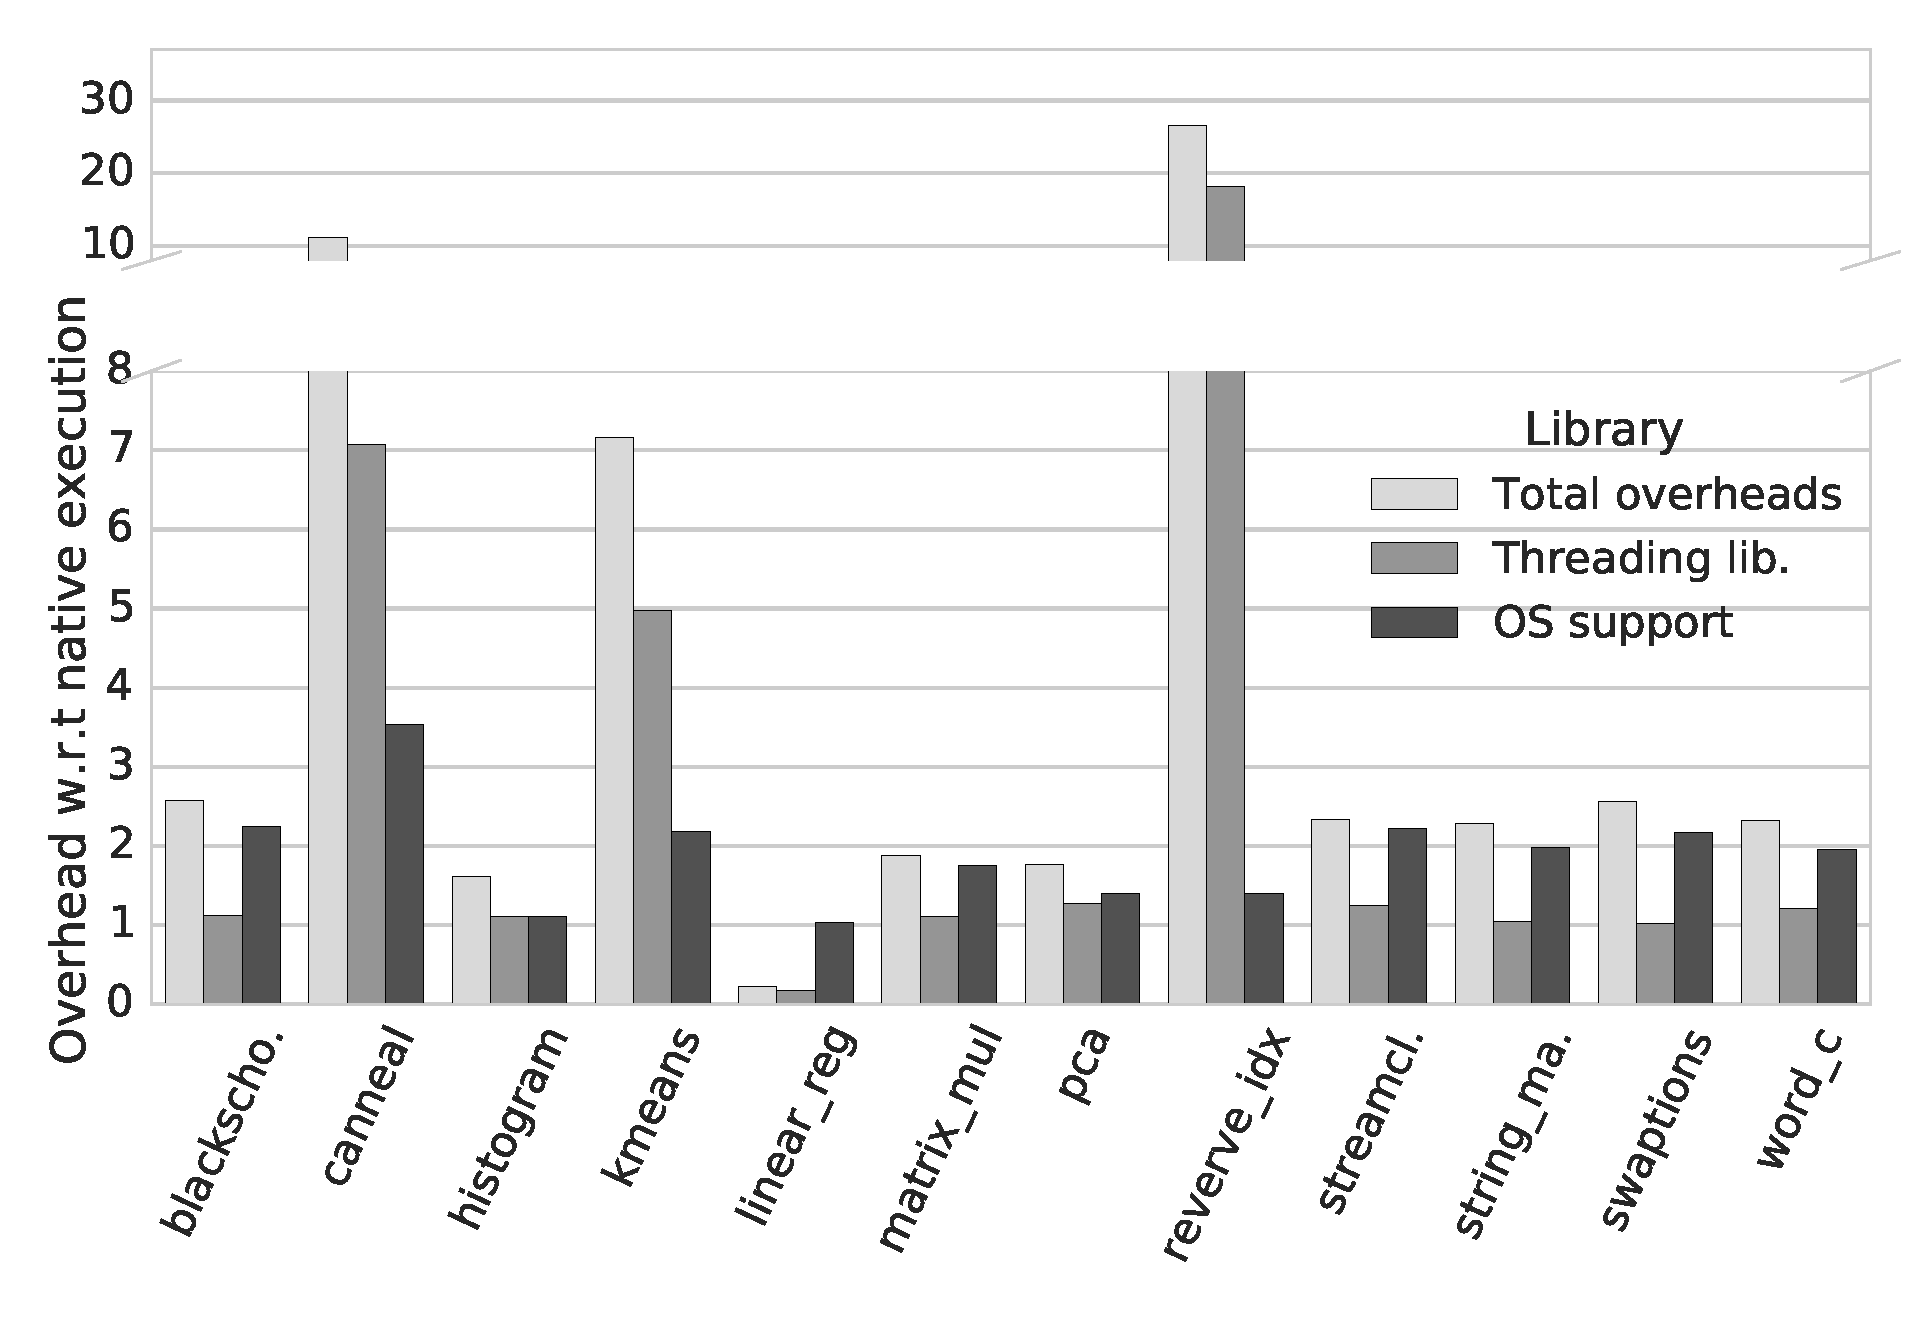
\includegraphics[scale=0.43]{figure/benchmarks/times-16-threads.pdf}
\caption{Performance overhead breakdown with $16$ threads --- except for streamcluster, where overhead for 15 threads is shown}
\label{fig:overheads-breakdown}
\end{figure}


\myparagraph{Additional results}   Due to the space limitation, the work measurements are available on the following: \href{https://mic92.github.io/inspector/index.html}{web-link}.

 %\href{https://goo.gl/0wp1kC}{Additional results Web-link.}

%In addition to time measurements, we also measured  {\em work} numbers, i.e., the overall CPUs utilization for all threads for both \pthreads and \projecttitle executions. (To measure work, we used the CPU accounting controller in {\tt cgroups} to account the CPU usage of all threads.)
%Due to the space limitation, we only present  time measurements for all experiments. 

%\myparagraph{Metrics: Time and Work}  We consider two types of measures to report the performance metrics: {\em time} and {\em work}. In a nutshell, time measurements reflect the end user perceived latency, whereas work measurements assess the overall resource (CPU) utilization.  More specifically,  time refers to the end-to-end computation time for the multithreaded applications. Work refers to the total computation performed by all threads, and it is measured as the cumulative CPU time for all threads. To measure work, we used the CPU accounting controller in {\tt cgroups} to account the CPU usage of all threads.

%\myparagraph{Measurements} All applications were compiled using GCC 5.2.1 compiler with -$o3$ optimization flag. For all performance measurements, we report the average over 10 runs with minimum and maximum values discarded.



\subsection{Provenance Overheads}
\label{subsec:overheads}
%First, we explain the provenance overheads imposed by \projecttitle w.r.t the native \pthreads execution.  We present the overheads with increase in: (1) the number of threads, and (2)  the input sizes.
First, we explain the provenance overheads imposed by \projecttitle w.r.t. the native \pthreads executions with increase in the number of threads. Figure~\ref{fig:overheads} shows the provenance overheads of \projecttitle w.r.t. the native \pthreads execution with varying number of
threads (from $2$ to $16$ threads). As expected, the provenance overheads increases with the increase in the number of threads. This is because the shared memory commit ($\S$\ref{sec:impl-lib}) takes longer time with a higher number of threads. 

The experiment shows that the provenance overheads using \projecttitle vary across applications. 
We observe that a majority of applications ($9$/$12$) have a reasonable overhead between $1\times$ up to $2.5\times$ w.r.t. the native execution. However, three applications have exceptionally high overheads:  {\em canneal}, {\em reverse\_index}, and {\em kmeans}. The high overheads is explained as follows: {\em canneal} modifies a lot of memory pages that leads to a high number of page faults for deriving read and write sets (see Table~\ref{tab:apps}). Whereas, {\em reverse\_index} does a lot of small memory allocations across threads leading to a large number of segmentation faults ($4241$ segmentation faults for memory allocation per second of the execution run-time, details omitted --- see  \href{https://mic92.github.io/inspector/index.html\#measurement_table}{web-link}).  Finally, {\em kmeans} creates more than $400$ threads until the cluster co-efficient converges, when we specify $500$ as the parameter for the iterative convergence algorithm (see Table~\ref{tab:apps}). Since, creating a process takes more time than creating a thread, we see a slowdown in {\em kmeans}.


On the other hand, {\em linear\_regression} performs better than \pthreads, which is explained by the fact that our implementation of threads as processes ($\S$\ref{sec:implementation})  avoids false sharing, as previously noted by Dthreads~\cite{dthreads-sosp-2011}, which leads to improved performance.



Lastly, in the case of {\em streamcluster}, we were limited by our physical memory to store the log in {\tt tmpfs} for $16$ threads (see $\S$\ref{subsec:overheads-breakdown}). Therefore, we also show the overheads with $14$ and $15$ threads,  where the provenance log can fit into the main memory.  To better understand the breakdown of provenance, we chose $15$ threads for {\em streamcluster} in $\S$\ref{subsec:performance-overheads-breakdown}.


%The overhead of collecting processor trace while using native
%\pthreads was 2 slower on average and there for causes an
%significant part of the of the slowdown.

%In {\tt Canneal} and {\tt Reverse Index} a high number of pages were modified.
%Reverse index does a lot of small memory allocations across the threads. This
%leads to more segmentation faults, because these allocations are located on
%different pages. In Kmeans during execution over 1000 threads were created. As
%processes take more time to create instead of threads, we see a slowdown here as
%well.
%
%For linear regression a speedup was measured. Because in this execution model,
%every “thread” has its own virtual memory: No cohearence protocol has to be run
%between commits. This prevents false sharing which results in a speedup even
%when recording the execution trace.

%The provenance overheads increases with the increase in the number of threads.
%This was expected, because the serial phase between memory commits takes longer,
%with a higher number of threads. 

%
%In Streamcluster, we were hitting the memory
%limit to store the log in {\tt tmpfs} for 16 threads. To better understand the
%breakdown we chose 15 threads in Figure~\ref{fig:overheads}, where the log can
%fit into the main memory. 


%\label{subsec:data-sizes-overheads}

\subsection{Performance overheads breakdown} 
\label{subsec:performance-overheads-breakdown}

Next, we investigated the breakdown of the provenance overheads. Recall that our system implementation has two major components: (1) the threading library ($\S$\ref{sec:impl-lib}), and (2) the OS support for \intelpt ($\S$\ref{sec:impl-OS}). 
Figure~\ref{fig:overheads-breakdown} shows the breakdown of overheads with $16$ threads normalized to the native \pthreads execution. We quantify the breakdown as the time taken by the \projecttitle library  and the OS support for \intelpt  . The result shows an interesting pattern: the applications with unreasonably high overheads ({\em canneal}, {\em reverse\_index}, and {\em kmeans}) spend a majority of time in the \projecttitle library for the above mentioned reasons. Whereas, the overheads for tracing the control flow due to \intelpt  is a dominant factor for the other applications. These results highlight that for a majority of applications ($9/12$) the underlying hardware is still a bottleneck to achieve low provenance overheads.  


\subsection{Scalability with input data}
\label{subsec:data-sizes-overheads}

\begin{figure}[t]
\centering
\myfontsize
{
\begin{tabular}{m{1.6cm}|m{3.4cm}| m{1.5cm}|m{1.4cm}}
   %   & & \multicolumn{2}{c|}{ Page faults }   &  Bandwidth & Branch instr. \\
   { Application} & Dataset / Parameters & Page fault & Page faults/sec\\
  \hline \hline
    blackscholes& 16 in\_64K.txt prices.txt &851& 57.3 \\
    canneal& 15 10000 2000 100000.nets 32 & 5343& 315.0 \\
    histogram& large.bmp & 381& 11.3  \\
    kmeans& -d 3 -c 500 -p 50000 -s 500 & 11900& 522.0  \\
    linear\_regression& key\_file\_500MB.txt & 183& 5.5  \\
    matrix\_multiply& 2000 2000 & 2101& 97.0  \\
    pca& -r 4000 -c 4000 -s 100 & 1900& 116.0\\
    reverve\_index & datafiles & 192& 5.7  \\
    streamcluster& 2 5 1 10 10 5 none output.txt 16 & 29300& 787.0\\
    string\_match &key\_file\_500MB.txt & 2751& 430.0\\
    swaptions & -ns 128 -sm 50000 -nt 16  & 7061& 929.0 \\
    word\_count& word\_100MB.txt	 & 4121& 508.0  \\

\hline
\end{tabular}
}


\caption{\label{tab:apps} Runtime statistics for all benchmarks with 16 threads (Detailed results are available here: \href{https://mic92.github.io/inspector/index.html\#measurement_table}{Log details web-link}) }                                                                                                                                  


\end{figure}

 In addition to scalability w.r.t.  threads, we also measured the performance overheads with increases in the size of the input.  For that, we
report the performance overheads for four applications that are available with
three input sizes: small ($S$), medium ($M$), and large ($L$). These four applications are: {\em histogram}, {\em linear\_regression}, {\em string\_match}, and {\em word\_count}.

In this experiment, we kept the number of threads to a constant  ($16$ threads), and we varied the input sizes for these applications.  Figure~\ref{fig:data-size-overheads} shows the results for our experiment. The bar plot shows the performance overheads w.r.t. to the native \pthreads execution on the $Y1$-axis for three input sizes ($S$, $M$, $L$). For the reference, the input sizes are also shown by a line plot in the same figure on the $Y2$-axis. 

The result shows that the gap between \pthreads and \projecttitle narrows with bigger input sizes. This is due to the fact that most applications use a data-parallel programming model for parallelization, where the main threads divides the input data evenly between the worker threads. As the input size increases, each thread needs to perform more work (or compute on a larger input size) than the time spend on synchronization. Therefore, in our implementation, each thread spends relatively more time outside the shared-memory commit to compute on the data, and therefore, it results in improved performance.
 

%
% algorithms used here divide input evenly between the
%threads. As the input size increase therefor the parallel phase increases and
%the overhead of the memory commit gets smaller in relatively.






%Next, we present  the sources for the provenance overheads. \projecttitle imposes two types of overheads: (1) performance overhead, and (2) space overhead for storing the provenance graph.





\subsection{Space overheads for provenance}
\label{subsec:overheads-breakdown}

Finally, we present the space overhead for storing the provenance graph. A major limitation of using \intelpt is that it produces a large amounts of trace data. Furthermore, the threading library also produces trace data to record the data and schedule dependencies.  Table~\ref{tab:space-overheads} shows the space overhead for all applications with~$16$ threads. Note that we report the combined space overheads for \projecttitle, the individual breakdown between the threading library and the OS support for \intelpt is available online:  \href{https://mic92.github.io/inspector/index.html\#measurement_table}{web-link}. 

The space overheads vary across applications: it can be as low as $183$ MB for {\em linear\_regression} and as high as $29.3$ GB for {\em streamcluster}. The result shows a strong correlation between the log bandwidth and branch instructions with a correlation coefficient of 0.89, which was expected, because the
log consists of taken branches.

Surprisingly,  the provenance log written by {\tt perf} turns out to be highly compressible. We
are able to achieve a compression ratio of between $6\times$ and $37\times$ times using the lz4 compression algorithm. 
Furthermore, the snapshot facility (described in $\S$\ref{sec:snapshot}) restricts the active area of space usage to $4$MB, and the user can reuse the space in the ring buffer after analyzing the log.



\begin{figure}[t]
\centering
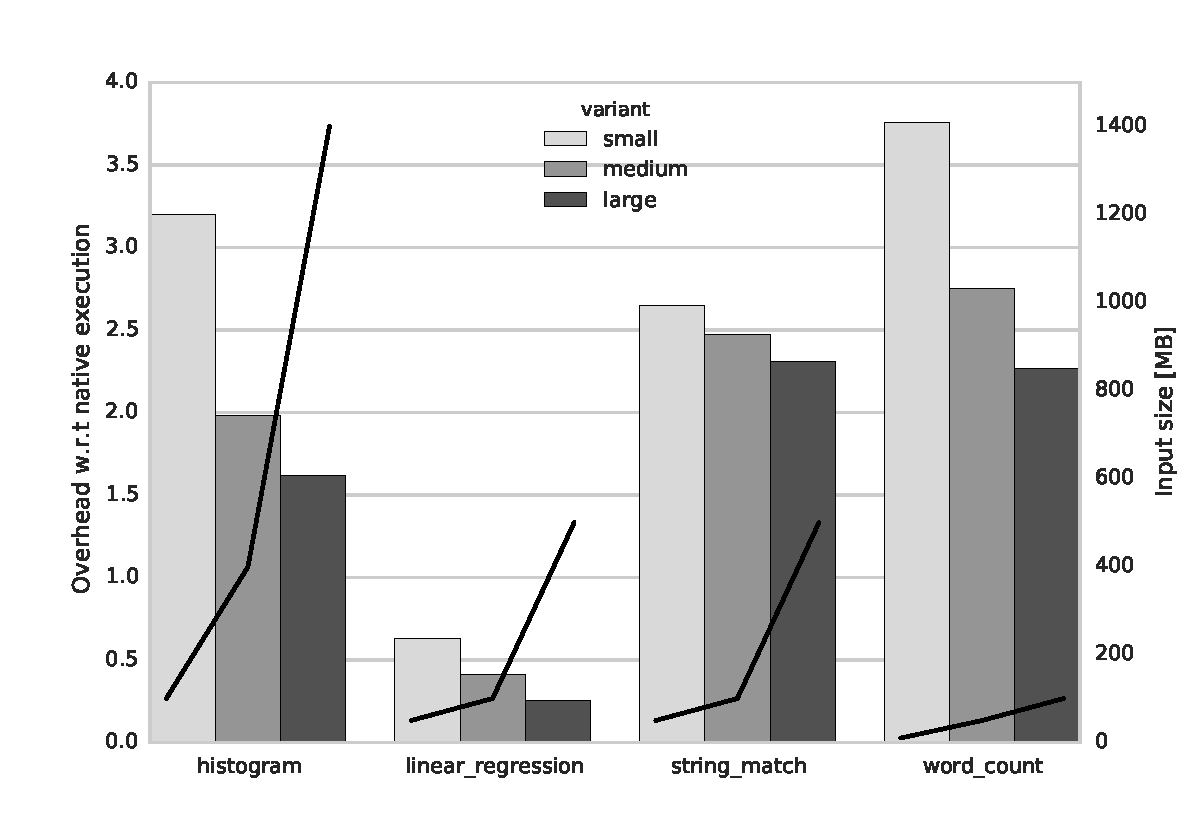
\includegraphics[scale=0.3]{figure/benchmarks/worksize-times-xy.pdf}
\caption{Scalability of overheads with increase in the input data sizes with $16$ threads. }
\label{fig:data-size-overheads}
\end{figure}





